\documentclass{article}
% https://github.com/Devinterview-io/docker-interview-questions
% Language setting
% Replace `english' with e.g. `spanish' to change the document language
\usepackage[english]{babel}


% Set page size and margins
% Replace `letterpaper' with `a4paper' for UK/EU standard size
\usepackage[letterpaper,top=2cm,bottom=2cm,left=3cm,right=3cm,marginparwidth=1.75cm]{geometry}
\usepackage[most]{tcolorbox}

\newtcolorbox{mybox}{
enhanced,
boxrule=0pt,frame hidden,
borderline west={4pt}{0pt}{green!75!black},
colback=green!10!white,
sharp corners
}
% Useful packages
\usepackage{amsmath}
\usepackage{graphicx, tcolorbox}
\usepackage[colorlinks=true, allcolors=blue]{hyperref}
\usepackage{xcolor}
\usepackage[dvipsnames]{xcolor}

\title{Kubernetes QnA}
\author{SS}

\begin{document}
\maketitle

\begin{abstract}
Your abstract.
\end{abstract}

\section{Introduction}

\begin{figure}
\centering
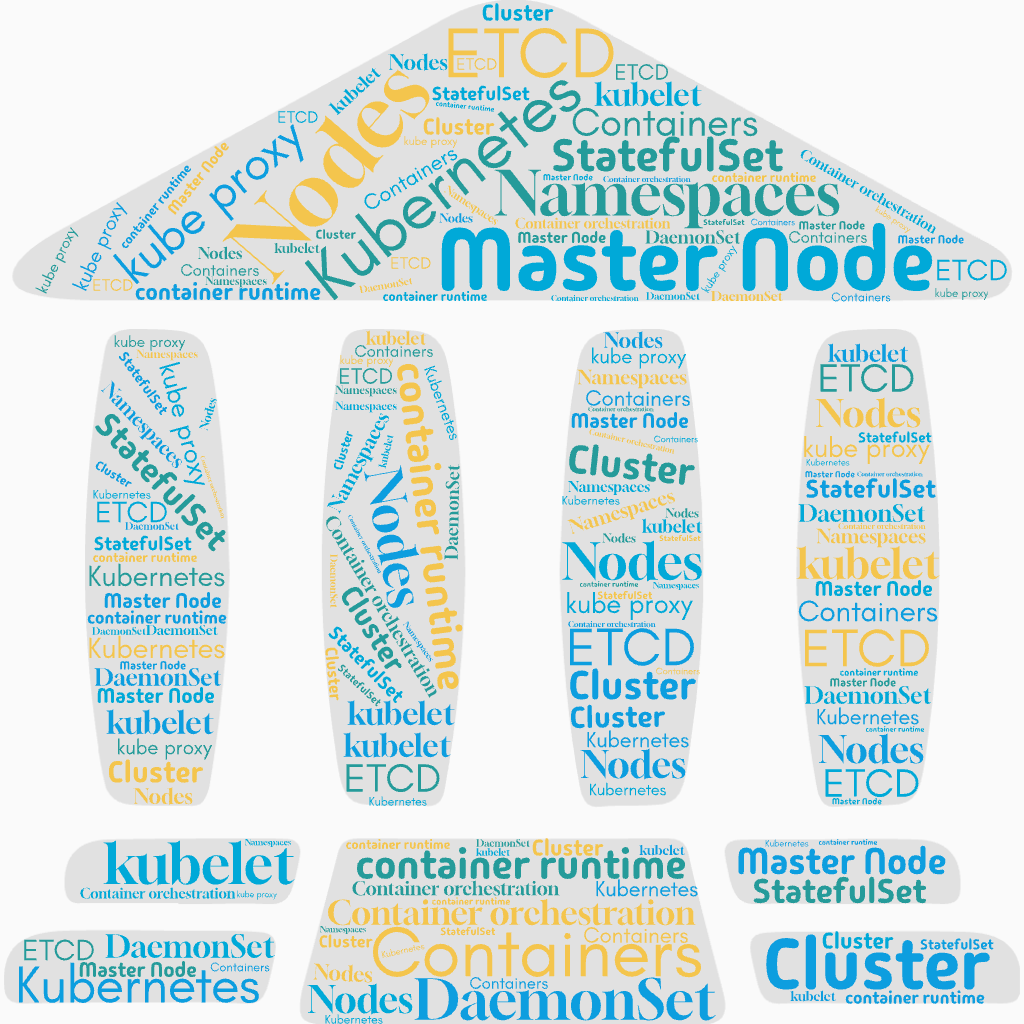
\includegraphics[width=0.95\linewidth]{k8sDiagrams/k8swordcloud.png}
\caption{\label{fig:k8s0}Kubernetes WordCloud.}
\end{figure} 

% 
%*********************************************************************
%*********************************************************************
\noindent
{\color{red} \rule{\linewidth}{0.5mm}}
\textcolor{red}{. What is a Kubernetes?} \\
\noindent
{\color{red} \rule{\linewidth}{0.5mm}}
Kuberenetes is an open source system for automating deployment, scaling and management of containerized applications. \\

\noindent
{\color{red} \rule{\linewidth}{0.5mm}}
\textcolor{red}{What is Kuberentes exactly ?} \\
\noindent
{\color{red} \rule{\linewidth}{0.5mm}}
 \\
 {\color{red} \rule{\linewidth}{0.5mm}}
\begin{tcolorbox}[colback=red!5!white, colframe=red!50!black,title=Kubernetes]
    The purpose of Kubernetes is to make it easier to organize and schedule your application across a fleet of machines. At a high level it is an operating system for your cluster. \\
\end{tcolorbox}
Basically, it allows you not to worry about what specific machine your datacentre each application runs on. Additionally, it provides generic primitives for health checking and replicating your applications across these machines, as well as services for wiring your application into micro-services so that each layer in your application is decoupled from other layers so that you can scale/update/maintain them independently. \\
%*********************************************************************
%                       K8s Pod
%*********************************************************************
\newpage
\section{Kubernetes Pod}
\noindent
{\color{red} \rule{\linewidth}{0.5mm}}
\begin{tcolorbox}[colback=red!5!white, colframe=red!50!black,title=What is a Kubernetes Pod?]
   \underline{\textit{A Kubernetes pod is a collection of one or more application containers.}} \\
A pod is additional level of abstraction that provides shared storage (volumes), IP address, communication between containers, and hosts other information about how to run application containers.\\
\textit{Containers do not run directly on virtual machines and pods are a way to turn containers on and off.}
\end{tcolorbox}
\begin{figure}
\centering
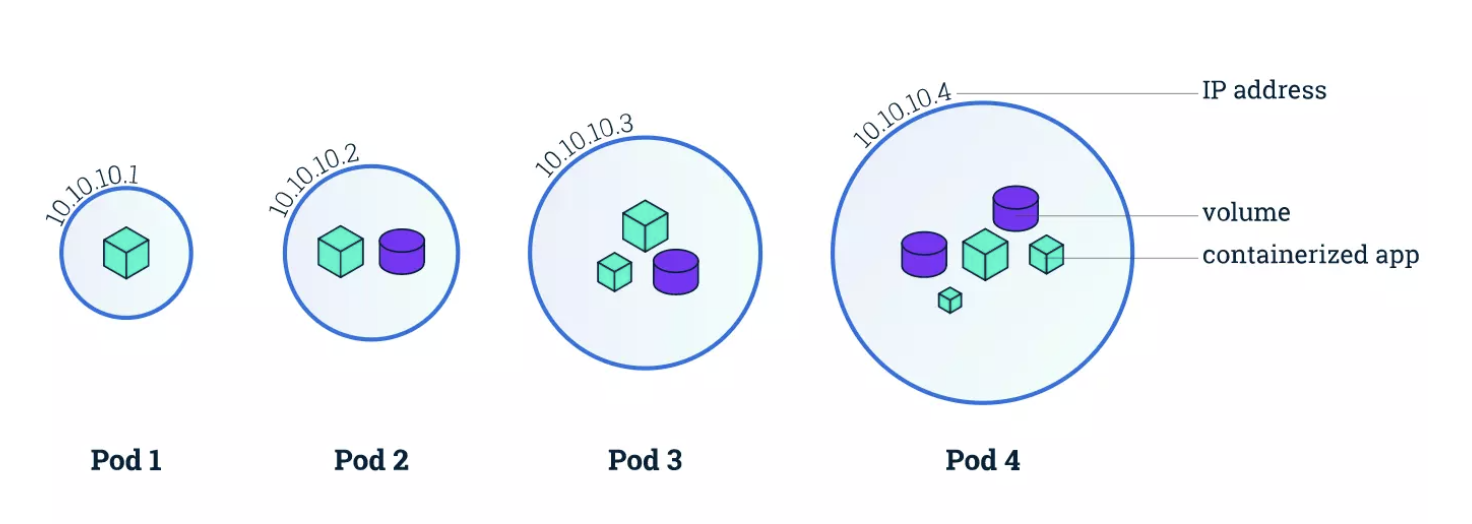
\includegraphics[width=0.95\linewidth]{k8sDiagrams/k8sPodArchi.png}
\caption{\label{fig:k8s1}Kubernetes Pod Architecture.}
\end{figure} 
Containers that must communicate directly to function are housed in the same pod. These containers are also co-scheduled because they work within a similar context. Also, the shared storage volumes enables pod to last through containers restarts because they provide consistent data. \\
Kubernetes also scales or replicates the number of pods up and down to meet changing load/traffic/demand/performance requirements. Similar pods scale together. \\
Also, \underline{\textit{when you create a kubernetes pod, the platform automatically schedules it to run on a \textbf{Node}}}. The pod will remain active until the specific process completes, resources to support teh pod run out, the pod object is removed, or the host node terminates or fails.\\
\textbf{Each pod runs inside a Kubernetes Node}, and each pod can fail over to another, logically similar pod running on a different node in case of failure.\\
\noindent
{\color{red} \rule{\linewidth}{0.5mm}}
\textcolor{red}{Explain what are some pod usage patterns} \\
\noindent
{\color{red} \rule{\linewidth}{0.5mm}}
Pods can be used in two main ways:
\begin{itemize}
    \item \textbf{ Pods that run a single containers}. The single and most common pod pattern is a single container per pod, where teh single container represents an entire application. In this case, you can think of pod as a wrapper.
    \item \textbf{ Pods that run multiple containers that need to work together}. Pods with multiple containers are primarily used to support co-located, co-managed programs that need to share resources. These co-located containers may form a single cohesive unit of service - one container serving files from a shared volume while another container refreshes or updates those files. The Pods wrap these containers and storage resources together as a single manageable entity. 
\end{itemize}
Each pod is meant to run a single instance of a given application. If you want to run multiple instances, you should use one Pod for each instance of the application. This is generally referred to as replication. Replicating pods are created and managed as a group by a controller, such as deployment. 

\noindent
{\color{red} \rule{\linewidth}{0.5mm}}
\textcolor{red}{How can containers within a pod communicate with each other ?} \\
\noindent
{\color{red} \rule{\linewidth}{0.5mm}}
Containers within a pod share networking space and can reach each other on local host. For instance, if you have two containers within a pod, a MYSQL container running on port 3306, and a PHP container running on port 80, the PHP container could access the MYSQL one through localhost:3306  \\
\noindent
{\color{red} \rule{\linewidth}{0.5mm}}
\textcolor{red}{What does a pod do ?} \\
\noindent
{\color{red} \rule{\linewidth}{0.5mm}}
Pod represents the processes running on a cluster. By limiting pods to a single process, Kubernetes can report on the health of each process running in the cluster. Pods have:
\begin{itemize}
    \item a unique IP address (whcih help them communicate with each other)
    \item persistent storage volume (as required)
    \item configuration information that determine how a container should run
\end{itemize}
Although most pods contain a single container, many will have a few containers that work closely together to execute a desired function.
\\
%*********************************************************************
%                       K8s Node
%*********************************************************************
\newpage
\section{Kubernetes Node}
\noindent
{\color{red} \rule{\linewidth}{0.5mm}}
\begin{tcolorbox}[colback=red!5!white, colframe=red!50!black,title=What is a Kubernetes Node?]
   \textit{A Kubernetes node is either a virtual or a physical machine that one or more Kubernetes pods run on.} \\
It is a worker machine that contains the necessary services to run pods, including the CPU and memory resources they need to run.\\
\end{tcolorbox}
\begin{figure}
\centering
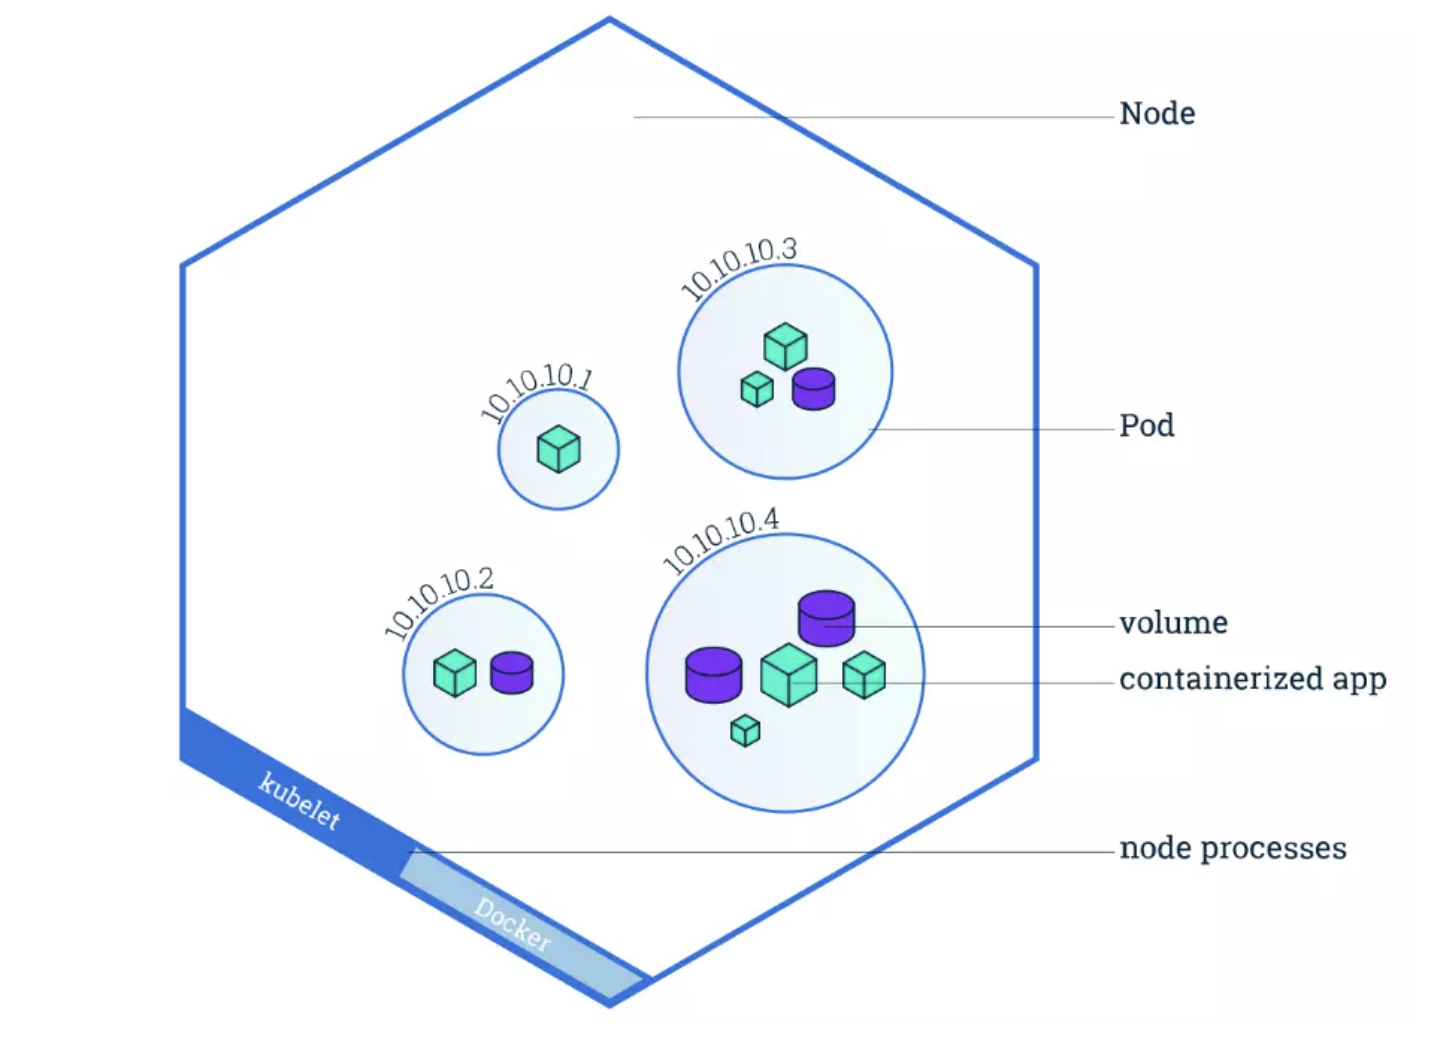
\includegraphics[width=0.85\linewidth]{k8sDiagrams/KubernetesNode.png}
\caption{\label{fig:k8sNode}Kubernetes Node.}
\end{figure} 
Each node comprises three crucial components:
\begin{itemize}
    \item \textbf{Kubelet} - This is an agent that runs inside each node to ensure pods are running properly, including communications between the Master and nodes.
    \item \textbf{Container runtime} - This is the software that runs containers. It manages individual containers, including retrieving container images from repositories or registries, unpacking them and running the application.
    \item \textbf{Kube-proxy} - This is a network proxy that runs inside each node, managing the networking rules within the node (between its pods) and across the entire Kubernetes cluster.
\end{itemize}

\begin{figure}
\centering
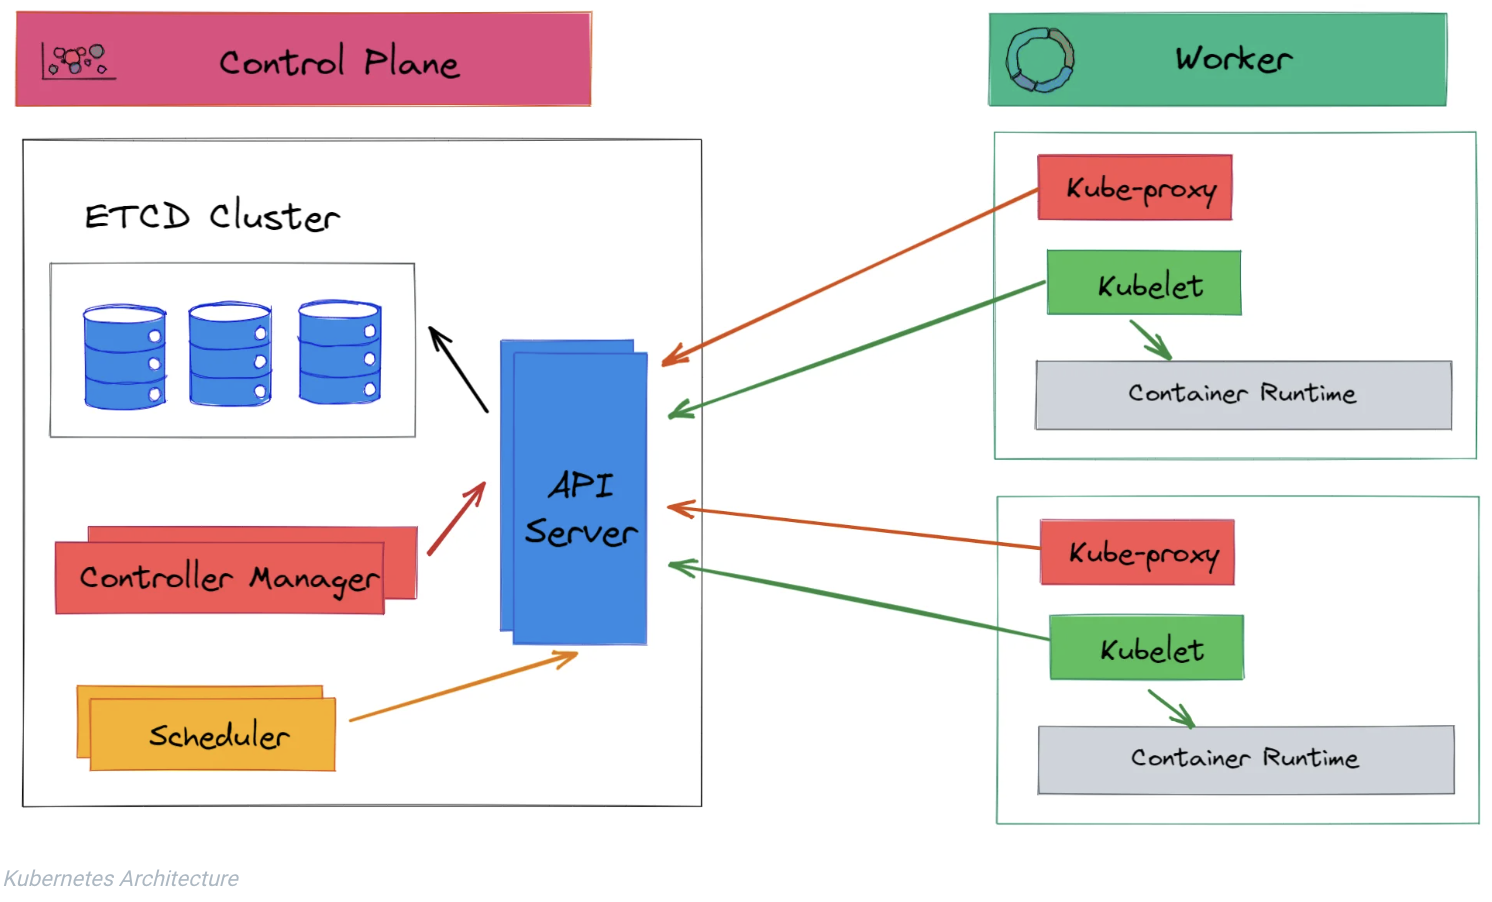
\includegraphics[width=0.95\linewidth]{k8sDiagrams/k8sArchitectureComponents.png}
\caption{\label{fig:k8sNode}Kubernetes Node.}
\end{figure} 


\noindent
{\color{red} \rule{\linewidth}{0.5mm}}
\textcolor{red}{Explain what is a Master Node and what component does it consist of?} \\
\noindent
{\color{red} \rule{\linewidth}{0.5mm}}
Pods can be used in two main ways:
\begin{itemize}
    \item The \textbf{ master node (Control Plane)} is the most vital component responsible for Kubernetes architecture.
    \item It is the central controlling unit of Kubernetes and manages workload and communication across the clusters. 
\end{itemize}
The master node (Control Plane) has various \textbf{  components}, each having its process. They are:
\begin{itemize}
    \item ETCD
    \item Controller Manager
    \item Scheduler
    \item API Server
\end{itemize}
\subsection{ETCD}
How can you ensure that your data is store consistently and reliably across a distributed system? Etcd is an open source key:value data store used to manage and store data that help keep distributed system running. Etcd is most well known for being a core component of Kubernetes. It stores and manages Kubernetes' State Data, Configuration Data and Meta Data. Etcd can be relied upon to being a single source of truth at any given point in time.  \\
What are the features of etcd that allow it to be so effective in this way? \\
etcd is :
\begin{enumerate}
    \item Fully \textbf{\textit{Replicated}}: every node in the etcd cluster has full access to the full data store.
    \item Reliably \textbf{\textit{Consistent}}: every data read in the etcd cluster is going to return the most reccent data write
    \item \textbf{\textit{Highly Available}}: There is no single point of failure in the etcd cluster. It can gracefully tolerate network partitions and hardware failure too. 
    \item \textbf{\textit{Fast}}: etcd is bench marked at 10000 writes/second. But that said, "etcd does persist data to disk". So etcd's performance is tied to your storage disk speed. 
    \item \textbf{\textit{Secure}}: Etcd uses transport layer security with optional SSL client certificate authentication.  Etcd stores vital and highly sensitive configuration data so it is important to keep it protected. 
    \item \textbf{\textit{Simple}} to use: A web application can read and writes data to etcd using simple http json tools. 
\end{enumerate}
\textit{etcd stores kubernetes \textbf{configuration} data and its \textbf{state} data}. etcd can use the \textbf{\textit{watch}} function to compare the configuration and state data. If they ever go out of sink, etcd will let the kubernetes API know and the kubernetes API will reconfigure the kubernetes cluster accordingly. \\
\textbf{\textit{Etcd can be used to store your data reliably and consistently across your distributed system. }}\\
The intended state of Kubernetes objects is saved in the etcd cluster for example when you create a pod.  In UNIX, all the \textbf{System Configuration Files} are stored in a directory called "etc". A "d" is augmented to "etc" to represent etcd's distribution model.\\
Etcd is reliable for cluster wide coordination and state management. Etcd is built on the top of Raft Algorithm. Raft gives etcd a total ordering of events across a system of distributed etcd nodes. This has many advantages and disadvantages.\\
The advantages are:
\begin{itemize}
    \item Any node may be treated like a master
    \item Minimal Downtime: a client can try another node if one isn't responding
    \item avoids split-braining
    \item a reliable way to build distributed lock for cluster-wide coordination
    \item users of etcd can build distributed systems without ad-hoc, buggy, homegrown solutions
\end{itemize}
For example, You would use etcd to coordinate an automated election of a new Postgres master so that there remains only one master in teh cluster. \\
The disadvantages are:
\begin{itemize}
    \item for safety reasons, it requires majority of teh cluster to commit writes - usually to disk - before replying to a client
    \item require more network chatter than a single master system. 
\end{itemize}
    
Distributed Key:Value Store. \\
The etcd cluster distributes the key:value information in a very reliable way. You can enter and read the data by Restful API or by some command line tools. The API server saves its intended state in the etcd cluster.
\textbf{ETCD}(Cluster Store)
\begin{enumerate}
    \item The component stores the configuration details and essential values.
    \item It communicates with all other components to receive the command and work in order to perform an action.
    \item It also manages network rules and posts forwarding activity.
\end{enumerate}
\noindent
{\color{red} \rule{\linewidth}{0.5mm}}
\textcolor{red}{How exactly is a Pod created?} \\
\noindent
{\color{red} \rule{\linewidth}{0.5mm}}
%*********************************************************************
%                       K8s Cluster
%*********************************************************************

\newpage
\section{Kubernetes Cluster}
\noindent
{\color{red} \rule{\linewidth}{0.5mm}}
\begin{tcolorbox}[colback=red!5!white, colframe=red!50!black,title=What is a Kubernetes Cluster?]
   Nodes usually work together in groups. \textit{A Kubernetes cluster contains a set of work machines (nodes).} The cluster automatically distributes workload among its nodes, enabling seamless scaling.

\end{tcolorbox}
\textbf{\textit{A cluster consists of several nodes}}. \underline{The node provides the compute power to run the setup.} It can be a virtual machine or a physical machine. A single node can run one or more pods. \\

Each pod contains one or more containers. A container hosts the application code and all the dependencies the app requires to run properly. \\

The cluster also comprise the \textbf{Kubernetes Control Plane (=Master)}, which manages each node within it. The control panel is a container orchestration layer where K8s exposes the API and interfaces for defining, deploying and managing container's life cycles. \\

The master asseses each node and distributes workloads according to available nodes. This load balancing is automatic, ensures efficiency in performance, and is one of the most popular features of Kubernetes as a container management platform. \\

You can also run Kubernetes cluster on Amazon's Elastic Kubernetes Service (EKS), Microsoft's Azure Kubernetes Service (AKS), or the Google Kubernetes Engine (GKE). \\
\begin{figure}
\centering
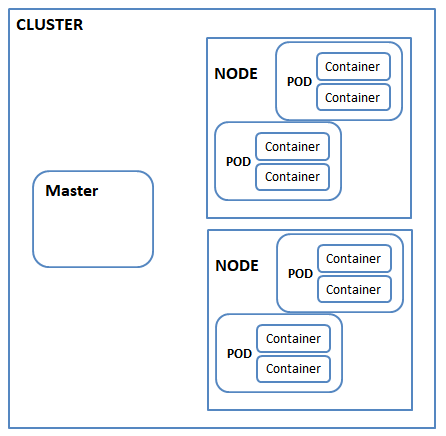
\includegraphics[width=0.5\linewidth]{k8sDiagrams/K8sCluster0.png}
\caption{\label{fig:k8sClusterComponents}Kubernetes Cluster Components.}
\end{figure} 
%*********************************************************************
%                       K8s Architecture
%*********************************************************************

\newpage
\section{Kubernetes Architecture}
\noindent
{\color{red} \rule{\linewidth}{0.5mm}}
\begin{tcolorbox}[colback=red!5!white, colframe=red!50!black,title= Kubernetes Architecture]
   Kubernetes groups fleets of machines in a logical unit called Kubernetes cluster. \underline{\textit{A Kubernetes cluster consists of the \textbf{control panel} and a set of worker machine called \textbf{nodes}}}. You can run many control plane components in a high availability mode. 
\end{tcolorbox}
\begin{figure}
\centering
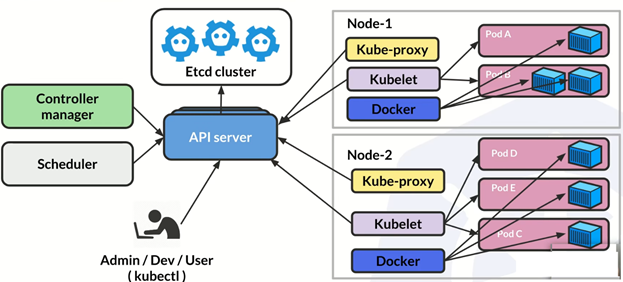
\includegraphics[width=0.95\linewidth]{k8sDiagrams/K8sClusterArchitecture.png}
\caption{\label{fig:k8sClusterArchi}Kubernetes Cluster Architecture.}
\end{figure} 
%*********************************************************************
%                       How to make a K8s Pod
%*********************************************************************

\newpage
\section{Kubernetes Pod Creation}
\noindent
{\color{red} \rule{\linewidth}{0.5mm}}
\textcolor{red}{How does Kubernetes create a Pod?} \\
\noindent
{\color{red} \rule{\linewidth}{0.5mm}}
When you make a Pod in Kubernetes what happens behind the scenes? How do the Kubernetes component work together to bring the pod into fruition? Let's go through the basics of Kubernetes from the perspective of a pod being made. The basis of our system is Node.The Nodes are the worker machine that back up the Kubernetes cluster. \\
In Kubernetes, there are 2 types of Nodes: 
\begin{enumerate}
    \item \textbf{Control Nodes}. In production level cluster, you would want at least three control nodes.
    \item \textbf{Compute Nodes}. One can have many Compute Nodes in a Kubernetes Cluster.
\end{enumerate}
Let's make a pod in Kubernetes.
\begin{enumerate}
    \item To make a pod in Kubernetes we use the \lstinline{kubectl} command. \item The \textbf{\lstinline{kubectl}} command will go into the Kubernetes Cluster and hit the \textbf{\lstinline{kube-API} Server}. The \lstinline{kube-API} Server is the main management component of a Kubernetes cluster. 
    \item  The first thing that the \lstinline{kube-API} server will do with the request to make a pod is to authenticate and validate the user. Check identity and access rights to the cluster. 
    \item  The \lstinline{kube-API} Server will then write that pod to the \lstinline{etcd}.  \lstinline{etcd} is a key:value data store that is distributed across the cluster. It is the source of truth to the Kubernetes cluster.
    \item \lstinline{kube-API} Server writes our request to etcd and the etcd then will return when it has made a successful write. 
    \item At that point the \lstinline{kube-API} Server will return to the user that the Pod is created. (even though not a lot has happened on the system yet). That is because, at its core Kubernetes and etcd have defined a desired state of what the system looks like and then all the Kubernetes components work together to make that desired state equal to the actual state. Now that we have the pod recorded in the desired state, it is as good as created. 
    \item The \textbf{scheduler} is keeping an eye on the workloads that need to be created and it will determine which node it will go on.
    \item What it is doing in the short term is that it is pinging our \lstinline{kube-API} Server at regular intervals (5s) to get a status of any workloads that need to be scheduled/created.
    \item Now that the scheduler knows that a pod needs to be created on one of the compute nodes .... 
    \item \textbf{Compute nodes have 3 major components}
    \begin{itemize}
        \item \textbf{Kubelet}. \textit{Kubelet is how the \textbf{compute node} communicates with the \textbf{Control Pane}, specifically the \lstinline{kube-API} Server}. Each compute node has a kubelet. \textit{kubelet is going to register the node with the cluster}. It will send periodic health check so that the \lstinline{kube-API} Server knows that the compute nodes are healthy.It will also create and destroy workloads as directed by the \lstinline{kube-API} Server. 
        \item \textbf{Container Runtime Engine/Initiative CRI / Docker}
        \item \textbf{kube proxy}: which is not needed to create the pod. \lstinline{kube-proxy} helps compute node communicate with each other if there are any workloads that span across more than one node. 
    \end{itemize}
    \item Scheduler is the where we need to schedule the new pod. Scheduler will look into the available compute nodes. It is going to rule out any that are unsatisfactory either because of limitations that may be the cluster administrator set up or there isn't any space for the pod. Of the ones that are left, it will choose the best one to run the workload on. Taking into account all the factors. 
    \item Once the Scheduler has made the choice, does it schedule the workload? No. All it does is tell the kube-API Server where it should go. 
    \item Once the kube-API server knows where it should go, does it schedule the workload? No. What the kube-API server does, is to write it to etcd. 
    \item Then after the successful write to the etcd, there is the desired state vs the actual state. The kube-API server then knows what it has to do to make the actual state meet the desired state.
    \item That's when the kube-API Server is going to know the respective kubelet (of the node ), to spin up a pod on this cluster. 
    \item The kubelet then will work together with the Container Runtime Engine and make a pod that has the appropriate container running inside.
    \item So now we have made a pod on Kubernetes Cluster. 
\end{enumerate}
One more management piece. Let's say when we created a pod, we \textit{set the restart policy to always}. Then let's say something happens and the pod goes down. \textit{How will the system know that a new pod needs to be created in its place?} That is where the \textbf{Controller Manager} comes in. The controller manager is made up of all the controllers. There are many controllers that are controlled by the controller manager. In particular, the one that is going to help us make the new pod. The \textbf{Replication Controller} within the controller manager will help with this task.  In the controller manager, all the different controllers are watching different pieces of the Kubernetes system. Just like the scheduler, these controllers in the Controller Manager are pinging the Kube-API Server at regular intervals to get an update on the actual state of the cluster to make sure that the desired state and actual state are same as one another. \\
The Replication controller by contacting the Kube-API Server sees that the pod is gone. It will then take the necessary steps to spin that pod back up. Rather create a new pod in its place. Because, \textbf{Pods are Ephemeral}. \\
In conclusion, all these components are working together just to make the pod. The Kube-API Server is the main management component of the cluster. Etcd is the data store and the source of truth for our cluster. The scheduler determines which of the compute node, the work node should go on to. The controller manager watches the actual state and makes sure that the actual state is the same as the desired state. 
%*********************************************************************
%                       Containers vs  Pod
%*********************************************************************

\newpage
\section{Kubernetes Pod Creation}
\noindent
{\color{red} \rule{\linewidth}{0.5mm}}
\textcolor{red}{Wjat is the difference between a container and a Pod?} \\
\noindent
{\color{red} \rule{\linewidth}{0.5mm}}
What are containers? Containers is a technology to package up an application (such as a webapp, a database, an API etc.) along with its 1. Code, 2. its Runtime and 3. its Libraries. It's everything that this application needs to run in an isolated environment which is packaged up in one singular unit. This unit is called a Container Image. \\
We take the container image and we can deploy it to a variety of different location such as a production server or another laptop/desktop etc.  It provides a standard for transporting and deploying applications. \\
What is the difference between containerisation technology and VM? They are both using virtualization. The VM includes the application, the library and the OS which can be pretty bulky at times. The container includes only the application and the library. It does not include the underlying OS. It uses the host's OS as well as its kernel and its resources in order to run the application. In effect, it is much more light weight, efficient and allows us to interact much faster when we are developing applications. \\
What containers really allow us to do is to create microservice based applications using Kubernetes. Kubernetes is the de facto standard in the orchestration of the containerized application. The allow us to manage, automate and to scale up/down the containerized applications in order to form one full application. \\
What are Kubernetes Pods?

%*********************************************************************
%*********************************************************************
%*********************************************************************
%*********************************************************************

\section{Reference}
\begin{itemize}
    \item \href{https://www.cloudzero.com/blog/kubernetes-node-vs-pod/}{Cloud Zero}
    \item \href{https://techdozo.dev/kubernetes-architecture/}{Techdozo}
    \item \href{https://www.youtube.com/watch?v=OmphHSaO1sE}{IBM Whiteny Lee}
    \item \href{https://www.fullstack.cafe/blog/kubernetes-interview-questions}{K8SQ\&A}
\end{itemize}
\end{document}